\section{Formalizing EARS using Linear Temporal Logic}

In this section we will use as running example the simplified requirements for
a controller for the engines of a (unspecified) machine. The machine includes a
\emph{main}, an \emph{auxiliary} and an \emph{oil pump} engine. The sequence to
start the machine is to first run the old pump engine; after 10 seconds start
the main engine; and finally after 5 more seconds start the auxiliary engine.
The \ears requirements for such a controller are depicted in
\fig\ref{fig:reqs_motor}.

\begin{figure}[!h]
\centering
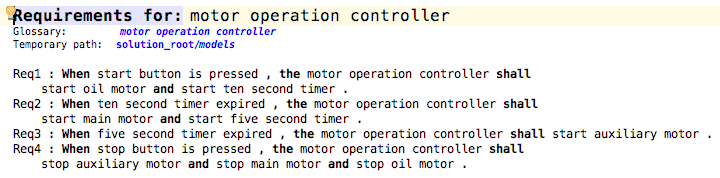
\includegraphics[width=.5\textwidth]{figures/motor_ears}
\caption{\ears requirements expressed in the \earsctrl tool}
\label{fig:reqs_motor}
\end{figure}

Let us now build a set of \ltl formulas that reflect the semantics of these
requirements. \ltl builds on propositional logic by adding temporal operators to
it. Formulas in \ltl are particularly appropriate to express properties of
runs of a reactive system, meaning how the state of that system should evolve
over time. For example, one may want to state that always when a motor is on,
then a thermostat is measuring its temperature. Or that, while the start button
is pressed then the starter engine will attempt to run the main engine. Or
even, that eventually the motor will stop. \ltl incorporates operators to
describe these situations. Due to space limitations we will not
formally introduce \ltl here, but will rather explain the formulas that we
introduce via our running example.

If we now turn our attention the example in 


\begin{itemize}
  \item A specification of a motor controller in EARS-CTRL
  \item Simple introduction to LTL
  \item Naive transformation of the motor requirements into LTL
\end{itemize}